\section{Image processing}
\begin{itemize}
	\item Apply various algorithms on image to analyze/improve the data
	\item The simplest kind of image transformation are those independent to the spatial position (thus also called point processing) where the new image is calculated by $g=a\cdot t(f)+ b$. Examples: gamma correction ($\log x$ to boost small, black values more than high ones), histogram equalization
\end{itemize}
\subsection{Neighborhood processing}
\begin{itemize}
	\item The most common way to process an image is by applying filters on it. A filter is a linear weighted sum of local input values. 
	\item A convolution of image $I$ and a linear filter $h$ is calculated by $$I_{out} = I \ast h, \hspace{1mm} I_{out}(i,j) = \sum\limits_{k,l} I(i-k, j-l) \cdot h(k,l)$$
	\item Depending on the size of the filter, we might not be able to apply the filter on the pixels at the border. Thus, we extend the image to have the same output shape. Common padding methods are zero/black, mirror/copy edge or wrap around.
	\item There are a lot of different filters that can be applied on an image. Filters can for example also be used for translation if wanted/needed. 1D example: $\left[\begin{array}{ccc}
	0 & 0 & 1
	\end{array}\right]$
	\item In general, we distinguish between \textit{low}-pass filters (smoothing) and \textit{high}-pass filters (edge detection, sharpening). The frequency is thereby the change of pixel values, and the passed wavelengths describe to what the filters react the most. Note that there are also \textit{band}-pass filters (low-pass filter convolved with high-pass filter)
	\item For example, unicolor images stay mostly unchanged when they are processed by an low-pass filter. In contrast, applying a high-pass filter on such images leads to very low activations.
\end{itemize}
\subsubsection{Smoothing filters}
\begin{itemize}
	\item \textit{Box filter}: replace every pixel by the average of its neighborhood. 
	$$h = \frac{1}{9}\left[\begin{array}{ccc}
	1 & 1 & 1\\
	1 & 1 & 1\\
	1 & 1 & 1\\
	\end{array}\right]$$
	Convolving a box filter with itself results in a filter in a shape of a Gaussian
	\item \textit{Gaussian filter}: weight contributions of neighboring pixels by distance: $G_\sigma = \frac{1}{2\pi \sigma^2} e^{-\frac{(x^2 +y^2)}{2\sigma^2 }}$. A $3\times 3$ Gaussian with $\sigma=0.5$ has the following values:
	$$h= \left[\begin{array}{ccc}
	0.011 & 0.084 & 0.011\\
	0.084 & 0.619 & 0.084\\
	0.011 & 0.084 & 0.011\\
	\end{array}\right]$$
	Note that convolving a Gaussian with another Gaussian is again a Gaussian. Thus, we can separate a 2D Gaussian into two 1D filters which are sequentially applied on the image $\Rightarrow$ reduce computational effort from $n^2$ to $2n$.
	\item \textit{Sharpening filter}: reverses the process of smoothing by accentuates differences with local average
	$$h = \left[\begin{array}{ccc}
	0 & 0 & 0\\
	0 & 2 & 0\\
	0 & 0 & 0\
	\end{array}\right]-\frac{1}{9}\left[\begin{array}{ccc}
	1 & 1 & 1\\
	1 & 1 & 1\\
	1 & 1 & 1\\
	\end{array}\right]$$
	\item \textit{Median filter}: A non-linear filter that selects the median value in the kernel window. The advantage of this filter is that its robust against outliers (good for filtering out salt-and-pepper noise)
\end{itemize}
\subsubsection{Edge detection filters}
\begin{itemize}
	\item \textit{Simple gradient filter}: The simplest gradient/edge detector is in 1D: $h = \left[\begin{array}{cc}-1 & 1\end{array}\right]$ 
	\item \textit{Sobel filter}: a derivative filter that also takes nearby pixels into account for better approximation. $h_x$ detects vertical edges (gradients over $x$-direction) and $h_y$ detects horizontal edges.
	$$h_x = \left[\begin{array}{ccc}
	1 & 0 & -1\\
	2 & 0 & -2\\
	1 & 0 & -1\\
	\end{array}\right] \text{\hspace{5mm}and\hspace{5mm}}h_y = \left[\begin{array}{ccc}
	1 & 2 & 1\\
	0 & 0 & 0\\
	-1 & -2 & -1\\\end{array}\right] $$ 
	\item \textit{Derivative of a Gaussian}: the derivative of a Gaussian is highly suitable for edge detection as it represents a band-pass filter (Gaussian filter convolved with discrete gradient filter although derivative mostly calculated by continuous). Similar to sobel, but weights the pixels nearby a bit different. Note that we also have different filters for $x$ and $y$ direction.
	\item \textit{Laplacian of Gaussian}: Laplacian operator $\nabla^2 f = \frac{\partial^2 
	f}{\partial x^2} + \frac{\partial^2 f}{\partial y^2}$ applied on a Gaussian. Is invariant to the direction of the gradient (circular symmetric). The shape of the function is also often described as a Mexican hat (see Figure~\ref{fig:cv_image_processing_gaussian_filters}). Is highly responsive to blobs (blob detection) but is sensitive to the scale. To be invariant of the scale, we can apply multiple LoG filters with different values of $\sigma$ and stack the results together.
	\begin{figure}[ht!]
		\centering
		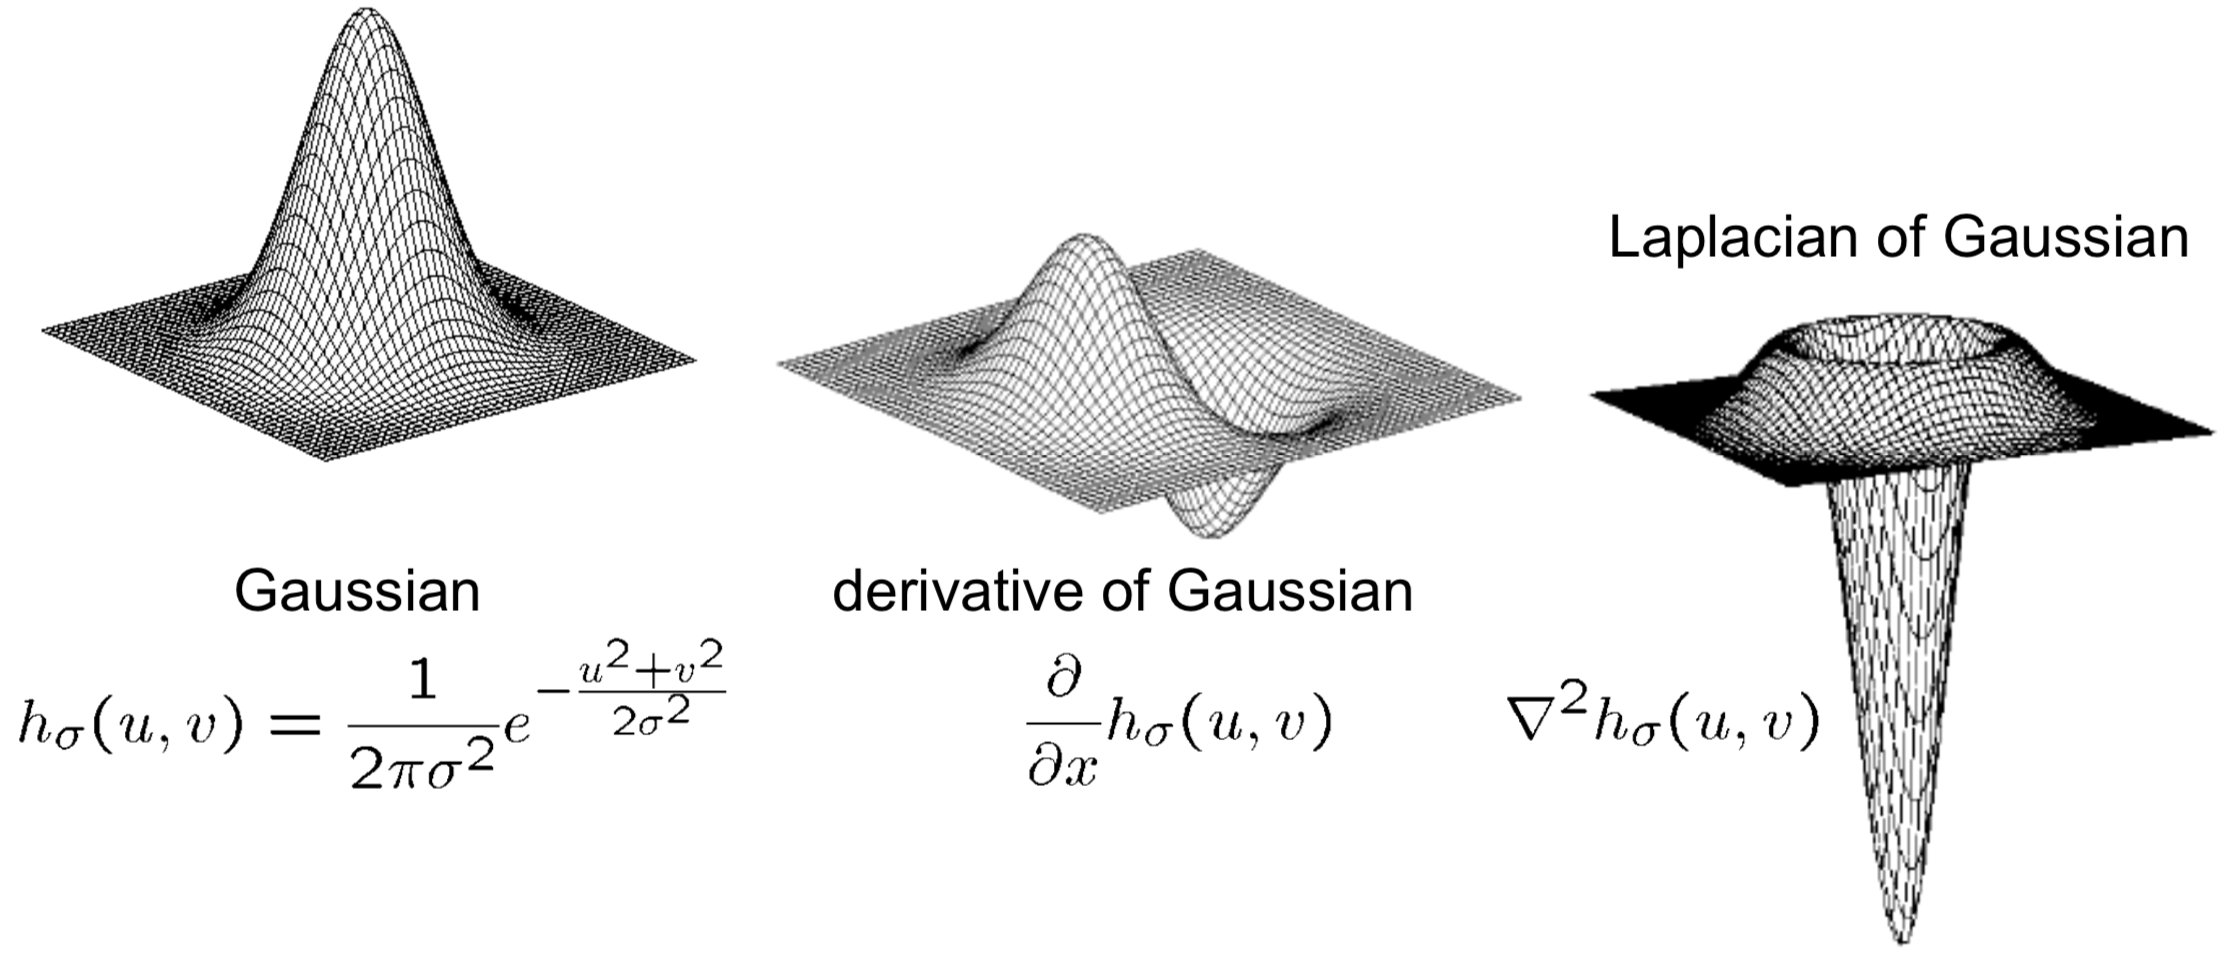
\includegraphics[width=0.6\textwidth]{figures/cv_image_processing_gaussian_filters.png}
		\caption{Visualization of different Gaussian filters.}
		\label{fig:cv_image_processing_gaussian_filters}
	\end{figure}
\end{itemize}
\subsection{Harris corner detector}
\begin{itemize}
	\item Detect interest points in an image to perform matching or similar tasks. Corners are suitable to serve as interest points as they have a unique 2D position compared to edges and points
	\item The initial idea is derived from performing autocorrelation on a small window of the image, and test which ones are unique/expressive. Now we are looking for small changes in $x$ and $y$ direction, how much the image changes. Based on that information, we can decide whether a pixel represents a corner or not.
	\item Steps in the Harris corner detector
	\begin{enumerate}
		\item Compute the derivatives $I_x$ and $I_y$ of the image
		\item Compute the products of the derivatives at every pixel: $I_x^2$, $I_y^2$, $I_{xy}=I_{x}\cdot I_{y}$ 
		\item Compute sums of products over the window size and align them in the Harris matrix:
		$$H = \left[\begin{array}{cc}
		\sum_W I_x^2 & \sum_W I_x \cdot I_y\\
		\sum_W I_x \cdot I_y & \sum_W I_y^2 \\
		\end{array}\right]$$
		Note that the sum represents the application of a box filter. It is equally possible to apply Gaussian filters etc. 
		\item Determine the response of the detector at each pixel:
		$$R = \det(H) - k\cdot \left(\text{trace}(H)\right)^2$$
		\item If $|R|$ is small, the region is probably flat. Otherwise, if $R<0$ (and greater a certain threshold) we have an edge, and $R>0$ indicates a corner.
		\item Perform non-maximum suppression if corner detector is calculated pixel-wise.
	\end{enumerate}
	\item Determining the \textit{cornerness} of a point is based on the eigenvalues of the matrix $H$: $R=\lambda_1 \lambda_2 - k\cdot (\lambda_1 + \lambda_2)^2$. The maximum eigenvalue is the gradient of the direction with the fastest change, and the minimum eigenvalue the gradient of the direction with the smallest change. Note that this models an ellipse for the gradients (see Figure~\ref{fig:cv_image_processing_harris_ellipse})
	\begin{figure}[ht!]
		\centering
		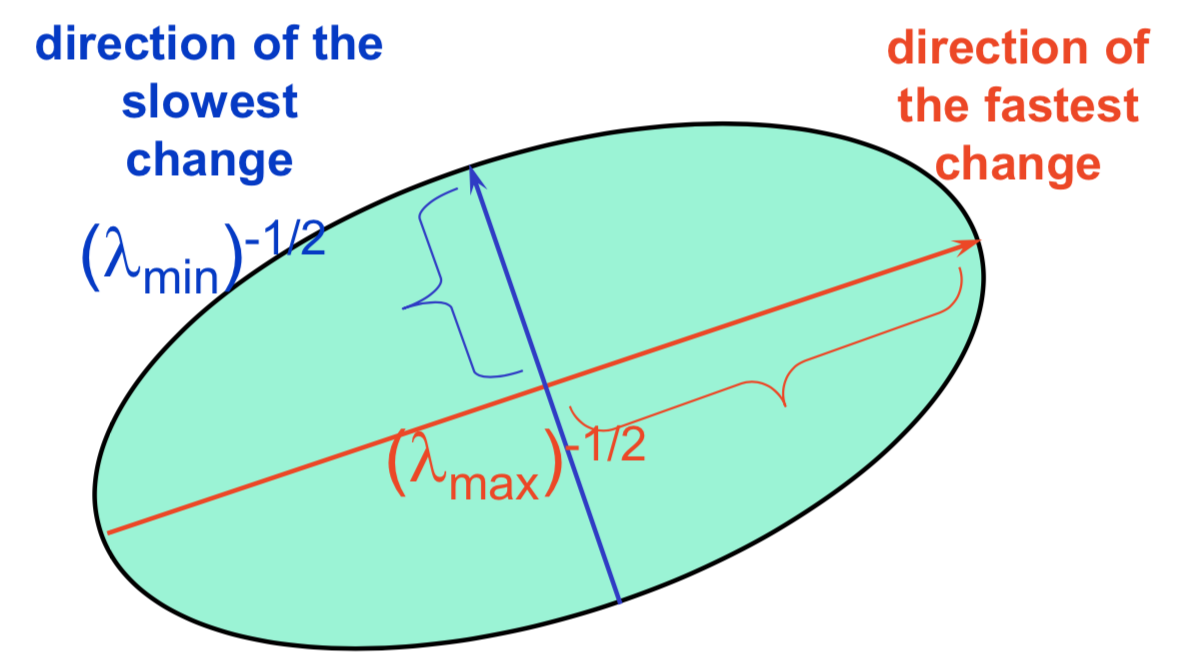
\includegraphics[width=0.25\textwidth]{figures/cv_image_processing_harris_ellipse.png}
		\caption{Visualization of relation between eigenvalues and gradients.}
		\label{fig:cv_image_processing_harris_ellipse}
	\end{figure}
	% cv_image_processing_harris_ellipse.png
	\item If we have an edge, one eigenvalue is considerably greater than the other as in one direction we have a large gradient, whereas in the other (90 degrees) the pixels stay the same. Here, $R$ is smaller than 0 as $\lambda_1\lambda_2$ is small but $\lambda_1 + \lambda_2$ is large.
	\item Thus, we only have a corner if in both directions we have a (equally) high change. In that case, $R$ is positive as $\lambda_1\lambda_2$ is large.
	\item Other properties of the Harris Corner detector
	\begin{itemize}
		\item Partial invariance to \textit{affine intensity} change. As only derivatives are used, a bias term $I+b$ does not influence result. When multiplying an image by a factor $I\cdot a$, we scale the eigenvalues and thus the cornerness as well. We therefore might only have to adapt the threshold.
		\item \textit{Rotation invariant} as only the ellipse rotates but the eigenvalues stay the same
		\item \textit{Scaling sensitive}: The Harris corner detector is sensitive to scale as it usually applies LoG/Derivatives of Gaussians for determining $I_x$ and $I_y$. To make the corner detector invariant to scale, we can apply multiple gradient filters with different values for $\sigma$ and stack them together (3D output instead of 2D). We then perform the detector on various scales, and take in the end the maximum response over scales for every pixel.
	\end{itemize}
	\item Applications
	\begin{itemize}
		\item \textit{Image stitching} as for combining separate photos into a panorama. We therefore detect interest points in all images, and try to match those (description by e.g. SIFT/histogram/...)
		\item \textit{Object recognition} by comparing local features that were found for a specific object with the ones from another image.
	\end{itemize}
\end{itemize}